\documentclass{article}

\PassOptionsToPackage{numbers,sort&compress}{natbib}
\usepackage{neurips_2026}

\usepackage[utf8]{inputenc}
\usepackage[T1]{fontenc}
\usepackage{hyperref}
\usepackage{url}
\usepackage{booktabs}
\usepackage{amsfonts}
\usepackage{amsmath}
\usepackage{amssymb}
\usepackage{nicefrac}
\usepackage{microtype}
\usepackage{xcolor}
\usepackage{graphicx}
\usepackage[inline,shortlabels]{enumitem}

\title{Router-R1-Local: Decomposition-Aware Routing Agents for Cost-Efficient Multi-LLM Reasoning}

\author{%
  Anonymous Authors \\
  Anonymous Institution \\
  \texttt{anonymous@neurips.cc}
}

\graphicspath{{../docs/static/figs/}{../figures/}}

\begin{document}

\maketitle

\begin{abstract}
Large language model (LLM) routing has mostly been treated as one-shot model assignment: given a query, dispatch it to one model and stop. This abstraction is too weak for complex questions whose solution requires decomposition, staged analysis, and different models at different steps. We propose \textbf{Router-R1-Local}, a \emph{decomposition-aware routing agent} that upgrades routing from passive dispatch to an agentic \emph{analyze-decompose-route-integrate} process. The key innovation is to make decomposition a first-class routing action: a small policy LLM decides whether a query should be answered directly or rewritten into two ordered sub-problems, routes each sub-problem to the most suitable external model, tracks intermediate sub-answers, and aggregates them into a final answer. The policy is trained with an agentic reinforcement-learning objective that jointly rewards answer quality, protocol validity, decomposition utility, and optional cost shaping, enabling the agent not only to improve answer quality but also to favor lower-cost model choices when cost-aware optimization is enabled. Because every routed step is explicit, the learned policy also induces an implicit top-k suitability ranking over the candidate model pool, revealing which models are preferred for different subproblem types. On seven question answering benchmarks, the released project artifacts show average exact-match gains from 0.338 to 0.416 over the strongest Qwen-based largest-model baseline and from 0.350 to 0.409 over the strongest Llama-based largest-model baseline. The released cost sweep further shows operating points that improve answer quality while reducing the proxy routing cost. These results support a new paradigm claim: complex multi-model QA should be handled by decomposition-aware routing agents rather than one-shot routers.
\end{abstract}

\section{Introduction}
\label{sec:intro}

Consider the question: \emph{what is the birth year of the actor who starred in \textit{Blood is Blood}?} A one-shot router would typically send the whole question to a single large model. Our local routing agent instead decomposes it into two smaller problems: identify the actor in \textit{Blood is Blood}, and then find that actor's birth year. In the released traces, these two steps can be solved by smaller models such as LLaMA-3.1-8B-Instruct and Qwen2.5-7B-Instruct, after which the agent integrates the intermediate answers into the final answer. A seemingly hard question is therefore transformed into a sequence of simpler, cheaper, and more controllable sub-questions.

Consider a second example: \emph{which university did Lee Smolin work at that is associated with causal dynamical triangulation?} Rather than treating this as a monolithic retrieval problem, the agent first identifies Lee Smolin and then answers the university question. In the local artifacts, both steps can be handled by LLaMA-3.1-8B-Instruct. This illustrates the central intuition of our project: a complex question often does not require one universally strongest model, but a policy that can analyze the question, expose its latent structure, and break it into lower-complexity subproblems that cheaper models can solve reliably.

These examples motivate a broader claim. Many hard QA problems become easier once the routing policy is allowed to \emph{decompose} before it \emph{routes}. This shifts the role of the routing model from simple model assignment to active problem solving. In our view, the routing model should not merely decide \emph{which} external model to call, but also \emph{whether} the original question should be decomposed, \emph{how} the decomposition should be structured, and \emph{when} enough evidence has been gathered to terminate.

\texttt{Router-R1-local} is our attempt to push LLM routing in that direction. Building on the reason-and-route idea of Router-R1 \cite{routerr1}, we introduce an explicit \textbf{decomposition-aware routing-agent paradigm}. The policy is no longer treated as a router that merely chooses among models; it is treated as a routing agent that can think, decide whether to decompose, call different external models for different sub-problems, emit intermediate sub-answers, and only then commit to a final answer. In the local branch, decomposition is intentionally constrained to a two-step linear execution plan. This design makes the agent's planning behavior explicit, keeps the action space manageable, and turns decomposition into a first-class part of the policy rather than an incidental prompting trick.

This new framing has three consequences that distinguish the project from Router-R1-style benchmark routing. First, decomposition becomes a capability primitive rather than an auxiliary behavior, so the agent can increase problem-solving power by transforming hard questions into answerable sub-questions. Second, because the policy is optimized with agentic RL and can include cost shaping, it can jointly learn \emph{which} model is most suitable and \emph{when} cheaper models are sufficient, producing a direct performance-cost trade-off rather than only a quality metric. Third, the routing trajectory itself becomes informative: repeated model choices over different subproblem types induce an implicit top-k ranking over the candidate model pool, so the routing agent also acts as a lightweight evaluator of model specialization.

The resulting system sits at the intersection of RL-trained reasoners such as DeepSeek-R1, tool-augmented agents such as Search-R1, cost-aware routers such as CARROT, and efficient RLHF infrastructure such as HybridFlow \cite{deepseekr1,jin2025search,somerstep2025carrot,sheng2024hybridflow}. Our claim, however, is more specific than ``multi-round routing works.'' We argue that explicit decomposition changes the nature of the problem: for complex queries, routing should be framed as an agentic control process over reasoning and model invocation, not as a one-shot classifier over a model pool. Relative to Router-R1, the local project emphasizes this shift by making decomposition ability explicit in the prompt protocol, the reward design, and the behavioral interpretation of the learned policy.

\paragraph{Contributions.}
We make four contributions. First, we advance a new \emph{routing-agent} viewpoint, in which model routing for complex questions is treated as an agentic process of deciding whether to decompose, how to solve sub-problems, and when to integrate answers. Second, we instantiate this viewpoint in \texttt{Router-R1-local} by introducing an explicit linear decomposition protocol with intermediate \texttt{<subanswer>} states, making decomposition a first-class capability of the routing policy. Third, we show that agentic RL can be used not only to improve answer quality but also to steer the policy toward lower-cost model choices through a controllable quality-cost trade-off. Fourth, we show that the resulting routing traces expose an implicit top-k preference structure over the model pool, turning the routing policy into a lightweight evaluator of model suitability across subproblem types.

\section{Method}
\label{sec:method}

\subsection{From router to routing agent}

Figure~\ref{fig:architecture} contrasts standard single-round routing with our multi-round alternative. In a single-round router, one policy directly maps the query to one target model. In Router-R1-Local, the policy first reasons about the problem, then decides whether it should be answered directly or rewritten into sub-problems, calls one or more external models, and integrates those outputs into later decisions. This is why we refer to the policy as a routing \emph{agent} rather than merely a router.

The local branch uses a strict protocol implemented directly in the prompting and evaluation code. If decomposition is used, it must create exactly two sub-questions in a linear execution plan. While the first sub-question is unresolved, the policy is not allowed to route the second one. This rule is important because it operationalizes the project's main novelty: decomposition is not free-form chain-of-thought, but an explicit control mechanism that structures the agent's future routing decisions.

This design creates a new systems abstraction. A traditional router solves ``which model should answer this query?'' Router-R1-Local instead solves ``should this query be decomposed, which model should answer each step, and when is enough information available to finish?'' That difference is the core paradigm shift of the local project.

Operationally, each episode starts from a user query $x$ and a candidate model pool $\mathcal{M} = \{m_1, \dots, m_K\}$. The routing agent maintains the query, the action-observation history, the current decomposition state, and the accumulated external-call cost. At every turn it may produce one of five structured actions: \texttt{<think>}, \texttt{<decompose>}, \texttt{<search>}, \texttt{<subanswer>}, or \texttt{<answer>}. The critical difference from ordinary routing is that \texttt{<decompose>} is a decision that changes the future control space. Once invoked, it creates two ordered sub-questions and turns the rest of the episode into a constrained multi-step process: only the current unresolved sub-question may be searched, solved, and marked done, and the final answer can only be emitted after all sub-questions are complete. In that sense, routing is no longer a one-shot classifier over models, but a sequential control policy over reasoning, model invocation, and termination.

We therefore optimize the routing agent at the trajectory level rather than the single-decision level. Let $\tau$ denote the full action trajectory for one query. The high-level objective is
\begin{equation}
J(\theta) = \mathbb{E}_{\tau \sim \pi_\theta}[R(\tau)],
\end{equation}
where $R(\tau)$ rewards both correct answering and efficient model usage. The local implementation uses token-level PPO with a KL penalty to a frozen reference policy, but the key modeling choice is that the return is defined over the entire decomposition-and-routing trajectory. As a result, the value of \texttt{<decompose>} is learned from its downstream effect on later searches, intermediate sub-answers, final accuracy, and total cost.

\begin{figure*}[t]
  \centering
  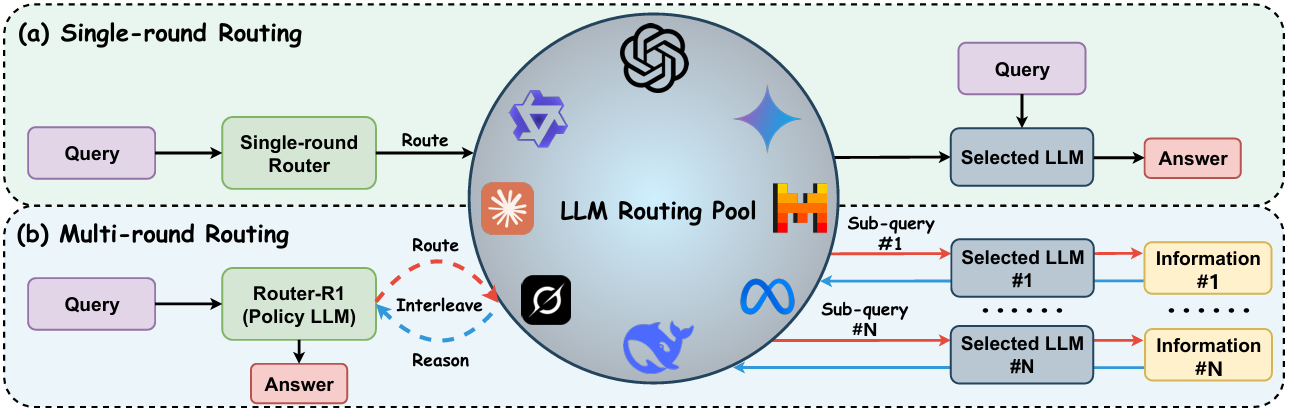
\includegraphics[width=0.95\textwidth]{model.png}
  \caption{Single-round versus multi-round routing. In Router-R1-Local, the policy LLM interleaves internal reasoning with external model invocation and can aggregate information across multiple routed sub-queries.}
  \label{fig:architecture}
\end{figure*}

\subsection{Task-conditioned model preference and implicit top-k evaluation}

The routing pool is configured through textual model descriptors rather than task-specific routing labels. The repository prompt template includes candidate models such as Qwen2.5-7B-Instruct, Llama-3.1-8B-Instruct, Llama-3.1-70B-Instruct, Mistral-7B-Instruct, Mixtral-8x22B-Instruct, and Gemma-2-27B-Instruct, along with short descriptions of their strengths. This design matters for generalization: the routing agent learns to make decisions from compact capability summaries rather than from a closed set of training-time model identities.

Because every \texttt{<search>} action explicitly names the chosen model, the learned policy induces a task-conditioned preference distribution over the model pool. Aggregating these choices across related subproblems yields an implicit top-k ranking of model suitability. We do not supervise such rankings directly; instead, they emerge from repeated decomposition-and-routing trajectories, which is why we view the agent not only as a solver but also as a lightweight evaluator of model specialization.

\subsection{Training objective and reward design}

The reward is where the decomposition-aware formulation becomes concrete. Rather than rewarding only the final answer, the local training loop scores the entire trajectory and explicitly credits useful decomposition behavior. The overall return is
\begin{equation}
R(\tau) = (1-\alpha) \bigl(R_{\mathrm{ans}}(\tau) + \bar{R}_{\mathrm{fmt}}(\tau)\bigr) + \alpha R_{\mathrm{cost}}(\tau) + R_{\mathrm{decomp}}(\tau),
\label{eq:reward_total}
\end{equation}
where $\alpha \in [0,1]$ controls the quality-cost trade-off.

The answer reward uses the hybrid objective implemented in the repository:
\begin{equation}
R_{\mathrm{ans}}(\tau) = \mathrm{EM}(y, y^*) + b_{\mathrm{F1}}\bigl(\mathrm{F1}(y, y^*), \mathrm{EM}(y, y^*)\bigr).
\label{eq:reward_answer}
\end{equation}
Here the exact-match score remains the main signal, while $b_{\mathrm{F1}}$ provides a bounded shaping bonus when the answer is close but not exactly correct. This matters in routing because partially correct intermediate trajectories are common during early learning, especially when the agent has identified the right decomposition but not yet the most reliable model for one of the sub-questions.

The format reward enforces the action grammar. Invalid tag structure, illegal nesting, malformed model queries, missing final answers, or violations of the linear decomposition protocol receive negative penalties. When the final answer is exactly correct, however, the local implementation clips the magnitude of the format penalty so that a correct trajectory is not dominated by a minor formatting defect. The cost reward is computed from the total expense of all external model calls in the trajectory and normalized into a cheapness-style score, so lower-cost trajectories receive larger $R_{\mathrm{cost}}$ values.

The main novelty lies in the decomposition reward, which directly values useful multi-step problem solving:
\begin{equation}
R_{\mathrm{decomp}}(\tau) = \mathrm{clip}\Bigl(
\lambda_{\mathrm{struct}} I_{\mathrm{struct}}
+ \lambda_{\mathrm{sub}} N_{\mathrm{sub}}
+ \lambda_{\mathrm{done}} I_{\mathrm{done}}
+ \lambda_{\mathrm{util}} U
- \lambda_{\mathrm{early}} I_{\mathrm{early}}
- \lambda_{\mathrm{unk}} I_{\mathrm{unk}}
\Bigr).
\label{eq:reward_decomp}
\end{equation}
In this expression, $I_{\mathrm{struct}}$ indicates that a valid two-step decomposition was produced, $N_{\mathrm{sub}}$ counts solved sub-questions, $I_{\mathrm{done}}$ indicates that all sub-questions were completed before the final answer, and $U$ is a utility bonus tied to final answer quality. The two negative terms penalize premature final answering before all sub-questions are resolved and low-information fallback answers such as unknown-style outputs. This term is important because it turns decomposition from an optional prompting behavior into a directly optimized capability.

Training uses PPO with KL regularization to a reference policy. To keep the presentation compact, we write the actor objective as
\begin{equation}
\mathcal{L}_{\mathrm{PPO}}(\theta) = \mathbb{E}_t \left[ \min\bigl(\rho_t A_t, \mathrm{clip}(\rho_t, 1-\epsilon, 1+\epsilon) A_t\bigr) \right],
\label{eq:ppo}
\end{equation}
where $\rho_t = \pi_\theta(a_t \mid s_t) / \pi_{\mathrm{old}}(a_t \mid s_t)$ and $A_t$ is computed from token-level rewards after applying a KL penalty against the reference policy. The important point for this paper is not the PPO variant itself, but that the policy gradient is taken with respect to whole decomposition-and-routing trajectories scored by Eq.~\ref{eq:reward_total}. As a result, the agent learns when decomposition improves answer quality, when smaller models are sufficient, and when additional external calls are not worth their cost.

More importantly, these routed decisions are themselves informative. When the policy repeatedly selects certain models for certain types of sub-questions, it is implicitly building a preference ordering over the model pool. In that sense, Router-R1-Local does not only answer questions; it also performs online evaluation of model suitability. The resulting traces can be aggregated into a task-conditioned top-k view of which candidate models are most useful for identification, temporal lookup, entity linking, or multi-hop synthesis.

\subsection{Reward design for agentic routing}

The answer reward in the local branch uses a hybrid exact-match and F1 design. Exact match remains the primary optimization signal. When exact match is zero but token-level F1 is sufficiently high, the policy may receive a capped shaping bonus. This avoids treating nearly-correct answers as equally bad as unrelated outputs.

Protocol validity is enforced through a hierarchical format reward. Severe violations such as malformed tags, illegal nesting, missing final answers, or invalid decomposition structure receive large penalties. Lesser mistakes, such as malformed model queries, receive smaller penalties. When the final answer is exactly correct, the implementation caps the negative impact of formatting errors so that a correct answer is not destroyed by an otherwise minor structural defect.

The local branch also adds a decomposition auxiliary reward. This term gives credit for creating a valid decomposition structure, solving sub-questions with concise \texttt{<subanswer>} actions, completing all sub-questions before the final answer, and using decomposition in a way that actually improves answer utility. The auxiliary term is bounded, which stabilizes training and prevents decomposition from dominating the learning signal.

Finally, the framework supports optional cost shaping. Cost is normalized into a cheapness-style reward so that lower-cost trajectories receive higher values. This is the mechanism by which the same agentic RL framework can move from pure capability learning to cost-aware model selection. The local documentation also makes clear that the current default run is accuracy-oriented, with \texttt{cost\_coe = 0.0}, and that the logged raw cost is an implementation-specific proxy rather than a full end-to-end dollar estimate. We therefore treat the cost analysis as a controlled quality-cost study rather than as a claim of exact monetary optimization.

\section{Experimental Setup}
\label{sec:exp}

\paragraph{Tasks.}
The repository evaluates on seven QA datasets: NQ, TriviaQA, PopQA, HotpotQA, 2WikiMultiHopQA, Musique, and Bamboogle. Following the released setup, training uses a mixed dataset built from NQ and HotpotQA, while the other benchmarks serve as out-of-domain evaluation.

\paragraph{Base policies.}
Two small policy backbones are studied: Qwen2.5-3B-Instruct and Llama-3.2-3B-Instruct. These models act as the routing agents. External queries are answered by candidate models in the routing pool.

\paragraph{Baselines.}
The released project compares against direct answering, chain-of-thought prompting, supervised fine-tuning, retrieval-augmented generation, Search-R1, prompt-based routers, the strongest single largest LLM, and several learned single-round routers such as RouterDC and GraphRouter.

\paragraph{Infrastructure.}
Training uses the veRL implementation of HybridFlow-style RLHF infrastructure \cite{sheng2024hybridflow}. The local repository exposes both evaluation scripts and an inference entry point that operates with the same structured action space used during training.

\section{Experimental Results by Innovation}
\label{sec:results}

\subsection{Decomposition turns hard questions into solvable subproblems}

Table~\ref{tab:main_results} summarizes representative results from the released project artifacts. For continuity with the repository naming, we retain labels such as Router-R1-Qwen and Router-R1-Llama in the table, but conceptually these models should be understood as our decomposition-aware routing-agent variants. They are consistently the strongest methods for both base policies. For Qwen2.5-3B-Instruct, the routing-agent variant reaches an average exact match of 0.416, exceeding the strongest non-Router-R1 baseline (Largest LLM, 0.338) by 7.8 points and Search-R1 by 12.5 points. For Llama-3.2-3B-Instruct, the corresponding routing-agent variant reaches 0.409 average exact match, improving over the Largest LLM baseline (0.350) by 5.9 points and over Search-R1 by 9.8 points.

The gains are not confined to a single data regime. The decomposition-aware routing-agent variant improves both in-domain performance on NQ and HotpotQA and out-of-domain performance on TriviaQA, PopQA, 2WikiMultiHopQA, Musique, and Bamboogle. This supports the paper's first innovation claim: explicit decomposition increases the effective problem-solving power of a small routing policy by converting complex questions into lower-complexity subproblems that the model pool can answer more reliably.

\begin{table*}[t]
\centering
\small
\setlength{\tabcolsep}{4.5pt}
\caption{Representative exact-match results on seven QA benchmarks from the released Router-R1 project artifacts. Dagger marks in-domain evaluation.}
\label{tab:main_results}
\resizebox{\textwidth}{!}{
\begin{tabular}{lcccccccc}
\toprule
\textbf{Method} & \textbf{NQ}$^\dagger$ & \textbf{TriviaQA} & \textbf{PopQA} & \textbf{HpQA}$^\dagger$ & \textbf{2Wiki} & \textbf{Musique} & \textbf{Bamboogle} & \textbf{Avg.} \\
\midrule
\multicolumn{9}{l}{\textbf{Qwen2.5-3B-Instruct as policy model}} \\
Direct & 0.092 & 0.260 & 0.122 & 0.140 & 0.266 & 0.026 & 0.040 & 0.135 \\
CoT & 0.126 & 0.358 & 0.160 & 0.168 & 0.208 & 0.046 & 0.224 & 0.184 \\
SFT & 0.212 & 0.400 & 0.160 & 0.198 & 0.256 & 0.052 & 0.112 & 0.199 \\
RAG & 0.298 & 0.540 & 0.366 & 0.216 & 0.146 & 0.078 & 0.224 & 0.267 \\
Search-R1 & 0.328 & 0.510 & 0.324 & 0.236 & 0.278 & 0.090 & 0.272 & 0.291 \\
Prompt LLM & 0.300 & 0.580 & 0.340 & 0.268 & 0.262 & 0.108 & 0.448 & 0.329 \\
Largest LLM & 0.296 & 0.578 & 0.354 & 0.278 & 0.274 & 0.104 & 0.480 & 0.338 \\
RouterDC & 0.278 & 0.592 & 0.282 & 0.244 & 0.218 & 0.080 & 0.504 & 0.314 \\
GraphRouter & 0.276 & 0.586 & 0.280 & 0.234 & 0.180 & 0.076 & 0.448 & 0.297 \\
\textbf{Router-R1-Qwen} & \textbf{0.388} & \textbf{0.706} & \textbf{0.384} & \textbf{0.352} & \textbf{0.434} & \textbf{0.138} & \textbf{0.512} & \textbf{0.416} \\
\midrule
\multicolumn{9}{l}{\textbf{Llama-3.2-3B-Instruct as policy model}} \\
Direct & 0.202 & 0.328 & 0.176 & 0.144 & 0.134 & 0.018 & 0.048 & 0.150 \\
CoT & 0.256 & 0.468 & 0.182 & 0.172 & 0.168 & 0.040 & 0.272 & 0.223 \\
SFT & 0.076 & 0.098 & 0.084 & 0.100 & 0.224 & 0.026 & 0.016 & 0.089 \\
RAG & 0.308 & 0.478 & 0.356 & 0.162 & 0.084 & 0.038 & 0.176 & 0.229 \\
Search-R1 & 0.372 & 0.578 & 0.360 & 0.282 & 0.226 & 0.084 & 0.272 & 0.311 \\
Prompt LLM & 0.304 & 0.638 & 0.374 & 0.248 & 0.198 & 0.132 & 0.528 & 0.346 \\
Largest LLM & 0.344 & 0.616 & 0.394 & 0.258 & 0.242 & 0.122 & 0.472 & 0.350 \\
RouterDC & 0.310 & 0.614 & 0.298 & 0.250 & 0.204 & 0.088 & 0.504 & 0.324 \\
GraphRouter & 0.316 & 0.602 & 0.290 & 0.222 & 0.170 & 0.084 & 0.416 & 0.300 \\
\textbf{Router-R1-Llama} & \textbf{0.416} & \textbf{0.680} & \textbf{0.432} & \textbf{0.322} & \textbf{0.368} & \textbf{0.128} & \textbf{0.520} & \textbf{0.409} \\
\bottomrule
\end{tabular}}
\end{table*}

\section{Cost-Aware Allocation and Behavioral Analysis}
\label{sec:analysis}

\subsection{Agentic RL enables quality-cost trade-offs}

The project also reports a cost-coefficient sweep for Router-R1-Qwen on four datasets. The key takeaway is not that one setting universally dominates, but that the same routing-agent policy class can move along a quality-cost frontier. For example, on PopQA, increasing the cost coefficient from $\alpha = 0.0$ to $\alpha = 0.6$ improves exact match from 0.384 to 0.414 while reducing the raw cost proxy from 98.3 to 75.9. On 2WikiMultiHopQA, the same change reduces the raw cost proxy from 150.8 to 113.8 while retaining a strong exact match of 0.422 compared with 0.434 at $\alpha = 0.0$. At the other extreme, $\alpha = 0.9$ sharply reduces the raw cost proxy to values around 5--7, but this comes with a substantial loss in answer quality. These patterns support the paper's second innovation claim: agentic RL can be used not only to learn better decomposition and routing behavior, but also to steer the policy toward lower-cost model choices.

\begin{figure*}[t]
  \centering
  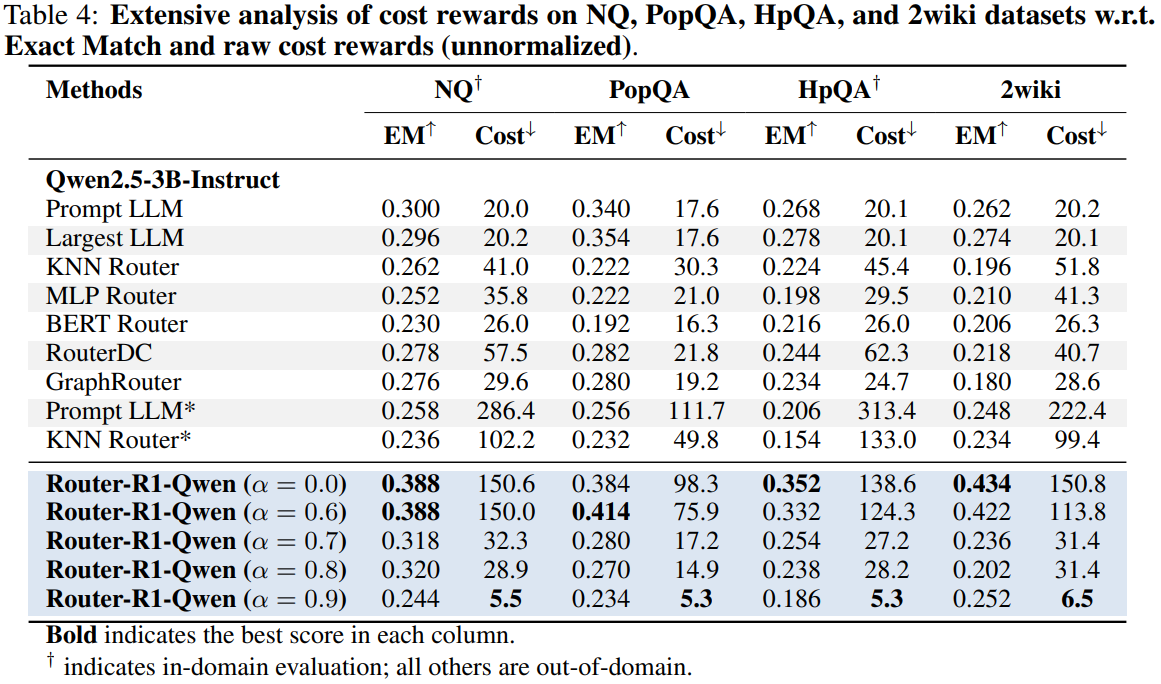
\includegraphics[width=0.92\textwidth]{cost.jpg}
  \caption{Cost-quality analysis from the released project page. Raw cost values are implementation-specific and are best interpreted as a relative proxy for routing expense rather than a full accounting of end-to-end monetary cost.}
  \label{fig:cost}
\end{figure*}

\subsection{Routing traces reveal implicit top-k model evaluation}

Figure~\ref{fig:behavior} provides two additional insights. First, the routing agent makes more external API calls on the multi-hop datasets 2Wiki and Musique than on single-hop datasets such as TriviaQA, which suggests that the learned policy adapts its use of external models to task complexity. Second, the training curves show that format reward is not merely cosmetic. With format reward enabled, reward rises smoothly and policy entropy declines in a stable manner; without it, training becomes unstable and eventually crashes. This is consistent with the local implementation, where invalid tag structure or illegal action sequences are heavily penalized.

Beyond call count, the trajectories also expose which models the agent prefers for which subproblem types. The local evaluation scripts explicitly summarize model usage counts, and a small trace analysis over a local decomposition artifact yields 31 analyzed decomposition cases, among which 5 already use more than one unique model in the same reasoning trajectory. In that artifact, the most frequently selected models are LLaMA-3.1-70B-Instruct (32 calls), Qwen2.5-7B-Instruct (10 calls), and LLaMA-3.1-8B-Instruct (10 calls). Qualitatively, the traces show the agent often routing lightweight factual identification and biographical lookups to 7B or 8B models, while reserving larger models for harder synthesis steps. This supports the paper's third innovation claim: the routing agent induces an implicit top-k preference structure over the model pool, so routing can also serve as a form of ongoing model evaluation.

\begin{figure*}[t]
  \centering
  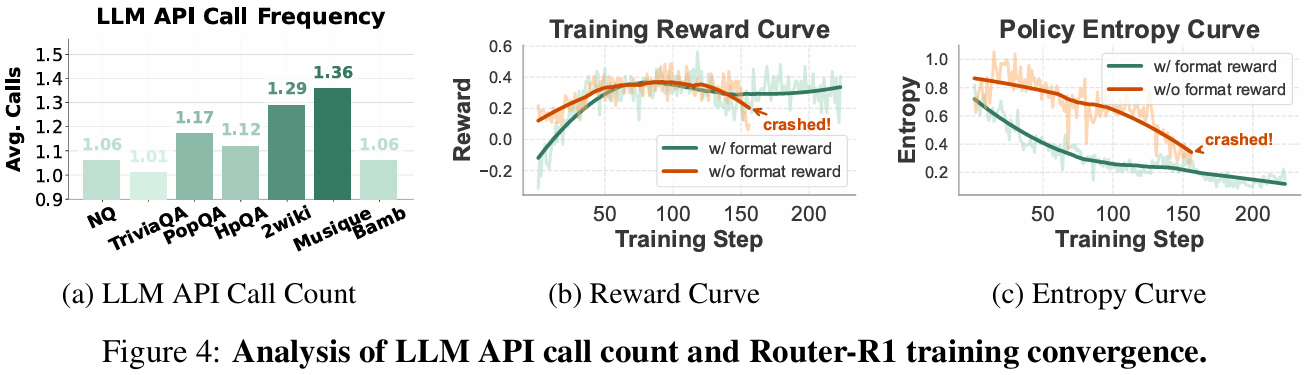
\includegraphics[width=0.92\textwidth]{discussion.jpg}
  \caption{Behavioral analysis from the released project page. Left: average number of external model calls by dataset. Middle and right: training reward and policy entropy with and without format reward.}
  \label{fig:behavior}
\end{figure*}

\section{Discussion}
\label{sec:discussion}

The results suggest a broader design lesson for LLM systems. A small model is often sufficient to control the \emph{process} of solving a problem even when it is not always the best model to produce every intermediate result itself. The main contribution of \texttt{Router-R1-local} is to make that process explicit as a routing-agent paradigm: the small policy model handles planning, decomposition, and control flow, while stronger external models are invoked only when the current sub-problem justifies the cost.

This perspective also clarifies why the local project should not be read as just another Router-R1 writeup. The point is not only that multi-round routing outperforms single-round routing, but that explicit decomposition changes what the policy is allowed to do, cost-aware agentic RL changes how the policy allocates model budget, and routed trajectories reveal which models are most suitable for which subproblems. The benefit is therefore not just model selection, but model selection \emph{conditioned on a decomposition-aware reasoning trajectory} that simultaneously improves capability, exposes efficiency trade-offs, and evaluates model specialization. In that sense, routing becomes an agentic control problem rather than a single-turn classifier.

\section{Limitations}
\label{sec:limitations}

This draft is grounded in the released \texttt{Router-R1-local} repository and its accompanying project page artifacts, which means its claims are only as strong as those artifacts. We did not regenerate every experiment from scratch inside this writing session.

The local branch also exposes several practical limitations that should be stated explicitly. First, decomposition is currently restricted to a linear two-step plan. This makes the action space easier to learn but rules out richer tree-structured reasoning. Second, the documented local run uses \texttt{cost\_coe = 0.0}, so the default training setup is accuracy-oriented rather than actively cost-optimized. Third, the repository's raw cost proxy is not a true end-to-end dollar cost: it is an implementation-specific normalized signal based on model pricing heuristics. Therefore, claims about ``lower cost'' should be interpreted as claims about a learned quality-cost trade-off within this framework, not as a universally calibrated financial guarantee.

Finally, the current evaluation focuses on question answering. It remains an open question how well the same routing protocol transfers to domains such as coding, long-form planning, or multimodal reasoning, where decomposition and verification may require different action grammars.

\section{Conclusion}
\label{sec:conclusion}

We presented \texttt{Router-R1-local} as more than a local reimplementation of Router-R1. Our central claim is that adding explicit decomposition ability transforms routing into a new \emph{routing-agent} paradigm for complex questions. In this paradigm, a small policy LLM does not merely choose a model; it analyzes whether the problem should be decomposed, routes each step to an appropriate external model, tracks intermediate sub-answers, and only then produces a final answer. This shift yields three linked benefits: better capability on complex questions through decomposition, better efficiency through cost-aware agentic RL, and an implicit top-k evaluation of model specialization through routed trajectories. The released artifacts show that this decomposition-aware formulation substantially improves exact-match accuracy over strong single-round routing and direct-answer baselines, while also exposing a tunable quality-cost frontier. More broadly, the project suggests that effective heterogeneous LLM systems may be built not by scaling a single monolithic model, but by training a compact controller that can decompose, route, evaluate, and integrate.

\bibliographystyle{plainnat}
\bibliography{references}

\appendix

\section{Implementation and Reproducibility Details}
\label{app:repro}

The repository documents a concrete reproduction path. The default software stack uses Python 3.9, PyTorch 2.4.0, vLLM 0.6.3, FlashAttention 2, and veRL. The project README provides explicit commands for data generation, training, evaluation, and inference. Training data is constructed by mixing 7K examples from NQ with 7K examples from HotpotQA, while evaluation covers seven QA benchmarks. The local reward-design document further records that the recent local run used \texttt{reward\_metric = hybrid} and \texttt{cost\_coe = 0.0}.

The project also exposes the task grammar used during training. The policy must begin with \texttt{<think>} and end with exactly one \texttt{<answer>}. When decomposition is used, it must generate exactly two ordered sub-questions and may only solve them in sequence through model-qualified \texttt{<search>} and concise \texttt{<subanswer>} actions. These rules are implemented both in prompting and in reward evaluation, which is why protocol correctness contributes directly to the training objective.

Open access is available through the released codebase, the linked Hugging Face collection for models and datasets, and the project page summarizing the main empirical results. In a real submission, authors should anonymize release links if double-blind review requires it.

\section{Additional Experimental Notes}
\label{app:expdetails}

The repository reports single released runs rather than a multi-seed statistical study. Accordingly, the paper reports point estimates for exact match and discusses trade-offs shown in the released figures, but it does not claim uncertainty estimates or hypothesis-test significance. This choice should be interpreted as a limitation of the currently available artifacts rather than as evidence that variance is negligible.

The training scripts indicate deployment on A100 80GB-style hardware for at least one local recipe, but the repository does not expose a trustworthy total-compute budget for the entire research cycle, including failed exploratory runs. We therefore treat compute disclosure conservatively in the checklist.

\section{Broader Impacts, Release Risks, and Asset Provenance}
\label{app:ethics}

The positive impact of this work is improved efficiency in heterogeneous LLM systems. If routing policies can solve simple questions with cheaper models and reserve expensive models for harder sub-problems, they can reduce the cost barrier for deploying strong QA systems. The main negative risk is that the same mechanism could make large-scale automated information systems cheaper to operate, including systems used for spam, low-quality content generation, or misleading automated assistance.

The codebase also introduces release considerations. Router-R1-style systems do not only answer questions; they decide which external models to call and how often to call them. Poorly constrained policies could increase API abuse, amplify unsafe outputs from underlying models, or optimize for low-cost but low-reliability answers in high-stakes settings. For that reason, the project should be deployed with task restrictions, provider-side rate limits, and careful logging of routed calls.

Regarding provenance, the local repository credits and builds on Router-R1, Search-R1, DeepSeek-R1, and veRL. The \texttt{Router-R1-local} repository itself is released under Apache-2.0. The paper also relies on public QA benchmarks and third-party model APIs; authors should verify and document the licenses and terms of service of each dataset and provider when preparing a final release package.

\input{checklist}

\end{document}